
\documentclass[a4paper]{article}
\usepackage[margin=2cm]{geometry}

\usepackage[utf8]{inputenc}
% \usepackage[polish]{babel}

\usepackage{color, colortbl}
\usepackage[dvipsnames]{xcolor}
\usepackage{listings}
\usepackage{graphicx}

\usepackage{setspace}

\usepackage{natbib}

\lstset{literate=%
{ą}{{\k{a}}}1
{ć}{{\'c}}1
{ę}{{\k{e}}}1
{ł}{{\l{}}}1
{ń}{{\'n}}1
{ó}{{\'o}}1
{ś}{{\'s}}1
{ż}{{\.z}}1
{ź}{{\'z}}1
{Ą}{{\k{A}}}1
{Ć}{{\'C}}1
{Ę}{{\k{E}}}1
{Ł}{{\L{}}}1
{Ń}{{\'N}}1
{Ó}{{\'O}}1
{Ś}{{\'S}}1
{Ż}{{\.Z}}1
{Ź}{{\'Z}}1,
language=c++,
keywordstyle=\color{gray},
commentstyle=\color{lightgray},
stringstyle=\color{lightgray},
numbers=left,
frame=TBlr,
breaklines=true,
tabsize=2,
numberstyle=\tiny,
basicstyle=\footnotesize \ttfamily
}

\renewcommand\thesection{\arabic{section}.}
\renewcommand\thesubsection{\thesection\arabic{subsection}.}
\renewcommand\thesubsubsection{\thesubsection\arabic{subsubsection}.}
\renewcommand\theparagraph{\thesubsubsection\arabic{paragraph}.}
\renewcommand\thesubparagraph{\theparagraph\arabic{subparagraph}.}

\title{Softcomputing \\ Translation system based on a Multilayer Perceptron: pictures of characters and digits into a Braille alphabet
signs - Report}
\author{\textbf{Krystian Horecki} 181079 \\ 
	\textbf{Antoni Buszta} 181013 \\
	Wroclaw Univeristy of Technology}
\date{15.11.2013 r.}

\begin{document}

\maketitle
\newpage
\onehalfspace

\section{Project description}
\subsection{Project goals} 
The goal of the project was to create autmatic translation mechanism from pictures of characters to Brail alphabet signs.
Pictures of the chanracters were supposed to be a source of input and training data for translation mechanism.
Translation engine was supposed to be created in form of Multilayer Perceptron which is kind of artificial neural network.
Important chalange was to create engine which allows to recognize and translate as many characters as it's possible and with many different disortions of dfferent levels.
There was no requirement to create user interface in order to focus on engine properties and results instead of good project appearance.
\subsection{Input data format}
Characters which were used as a source of inout data were presented in form of images which were converted to tables cointaining boolean values.
This convestion allowed us to make input data more friendly for further processing. At the same time data still contained exactly the same data as picture and could be converted to this form in any time.
Example table containing character of capital \textbf{A} was presented below. \\
\begin{center}
		[0, 0, 0, 0, 0, 0, 0, 0, 0, 0,\\
        0, 0, 0, 0, 0, 0, 0, 0, 1, 0,\\
        0, 0, 1, 1, 1, 1, 1, 1, 1, 0,\\
        0, 1, 0, 0, 0, 1, 0, 0, 1, 0,\\
        1, 0, 0, 0, 0, 1, 0, 0, 0, 0,\\
        1, 0, 0, 0, 0, 1, 0, 0, 0, 0,\\
        0, 1, 0, 0, 0, 1, 0, 0, 1, 0,\\
        0, 0, 1, 1, 1, 1, 1, 1, 1, 0,\\
        0, 0, 0, 0, 0, 0, 0, 0, 1, 0,\\
        0, 0, 0, 0, 0, 0, 0, 0, 0, 0]\\
\end{center}
 
\subsection{Translation mechanism}
As a translation mechanism Multilayer Perceptron was used. To create MP we used Python programming language and pyBrain library which allows to easily create neural network with required nodes configuration. Preparing project we were experimenting with following properties of network:
\begin{itemize}
	\item number of hidden layers
	\item number of neurons in hidden layer
	\item types of hidden layer
	\item types of output layer
	\item output data presentation methods
\end{itemize}
Results of those experiments were presensted later in this paper.

\subsection{Output data format}
During experiments we decided to check 2 different approaches of output data computing:
\begin{enumerate}
	\item \textbf{Translation:} Encoded Brail alphabet characters in form of table, one output neuron refers to one position in table 
	\item \textbf{Clasification:} One output neuron per one class, which means that each output neuron represents different Brail symbol
\end{enumerate}
Because those two methods mean that different number of output neurons are used they can give different translation results.
Results of testing those two approaches were presented later in this paper.

\section{Used preprocessing and postprocessing methods}
\subsection{Preprocessing} 
To make network more sensitive to black and white pixels which are presented in input data as 0 and 1 we made function converting all zeroes to -1.
It allowed to imporove learning and testing results irrespective of output data computation method(clasification or direct translation).
\subsection{Postprocessing}
In case of postprocessing, used method deppended on output data computation method, which means that two different postprocessing methods were used:
\subsubsection{Translation postprocessing method}
Postprocessing was based on assumption that neural network output was in form float numbers table.
To create final result we rounded those numebrs to 1 or 0 which gave us proper result.
\subsubsection{Clasification postprocessing method}
During clasification neural network as a result gives us table of float numbers with values reffering to different classes of output data.
To decide which class is a proper one we used method choosing the biggest value from the table. The index of the biggest value was used to determine final class of object recognized by neural network. 

\section{Training sets and methods}
As a training set the pool of capital letters was used. Each letter was represented in set 300 times to make it easier to learn network. During preparations few tests for optimal learning were done with following properties as a variable:
\begin{itemize}
	\item Learning epochs number
	\item Number of hidden neurons
	\item Learning rate
	\item Momentum - value for parameters of network are adjusted
\end{itemize}

On figure \ref{epochs} it can be seen how avarage number of maximum noisy pixels changes along with number of training epoch. Network behaviour was tested wih both translation and clasification methods, which also can be seen on chart.
\begin{figure}[h!]
	\centering
	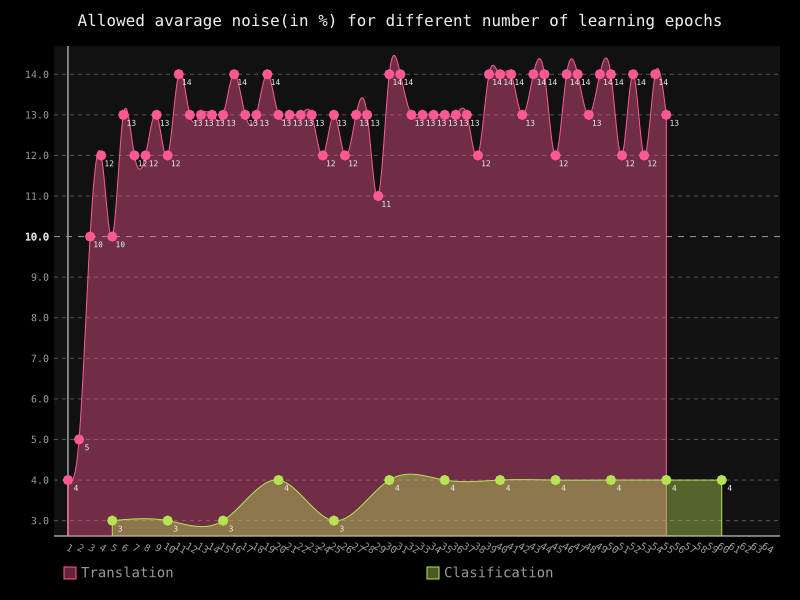
\includegraphics[scale=0.7,keepaspectratio=true]{Charts/epochsChart.png}	
	\caption{}
	\label{epochs}
\end{figure}
After tests we decided to use 55 training epochs to provide sufficient training level for network.
It was also tested how number of hidden neurons affects results of characters recognition.
As it can be seen on figure \ref{hidden} that relatively good results we get with 55 hidden neurons so this number was later used for tests.
\begin{figure}[h!]
	\centering
	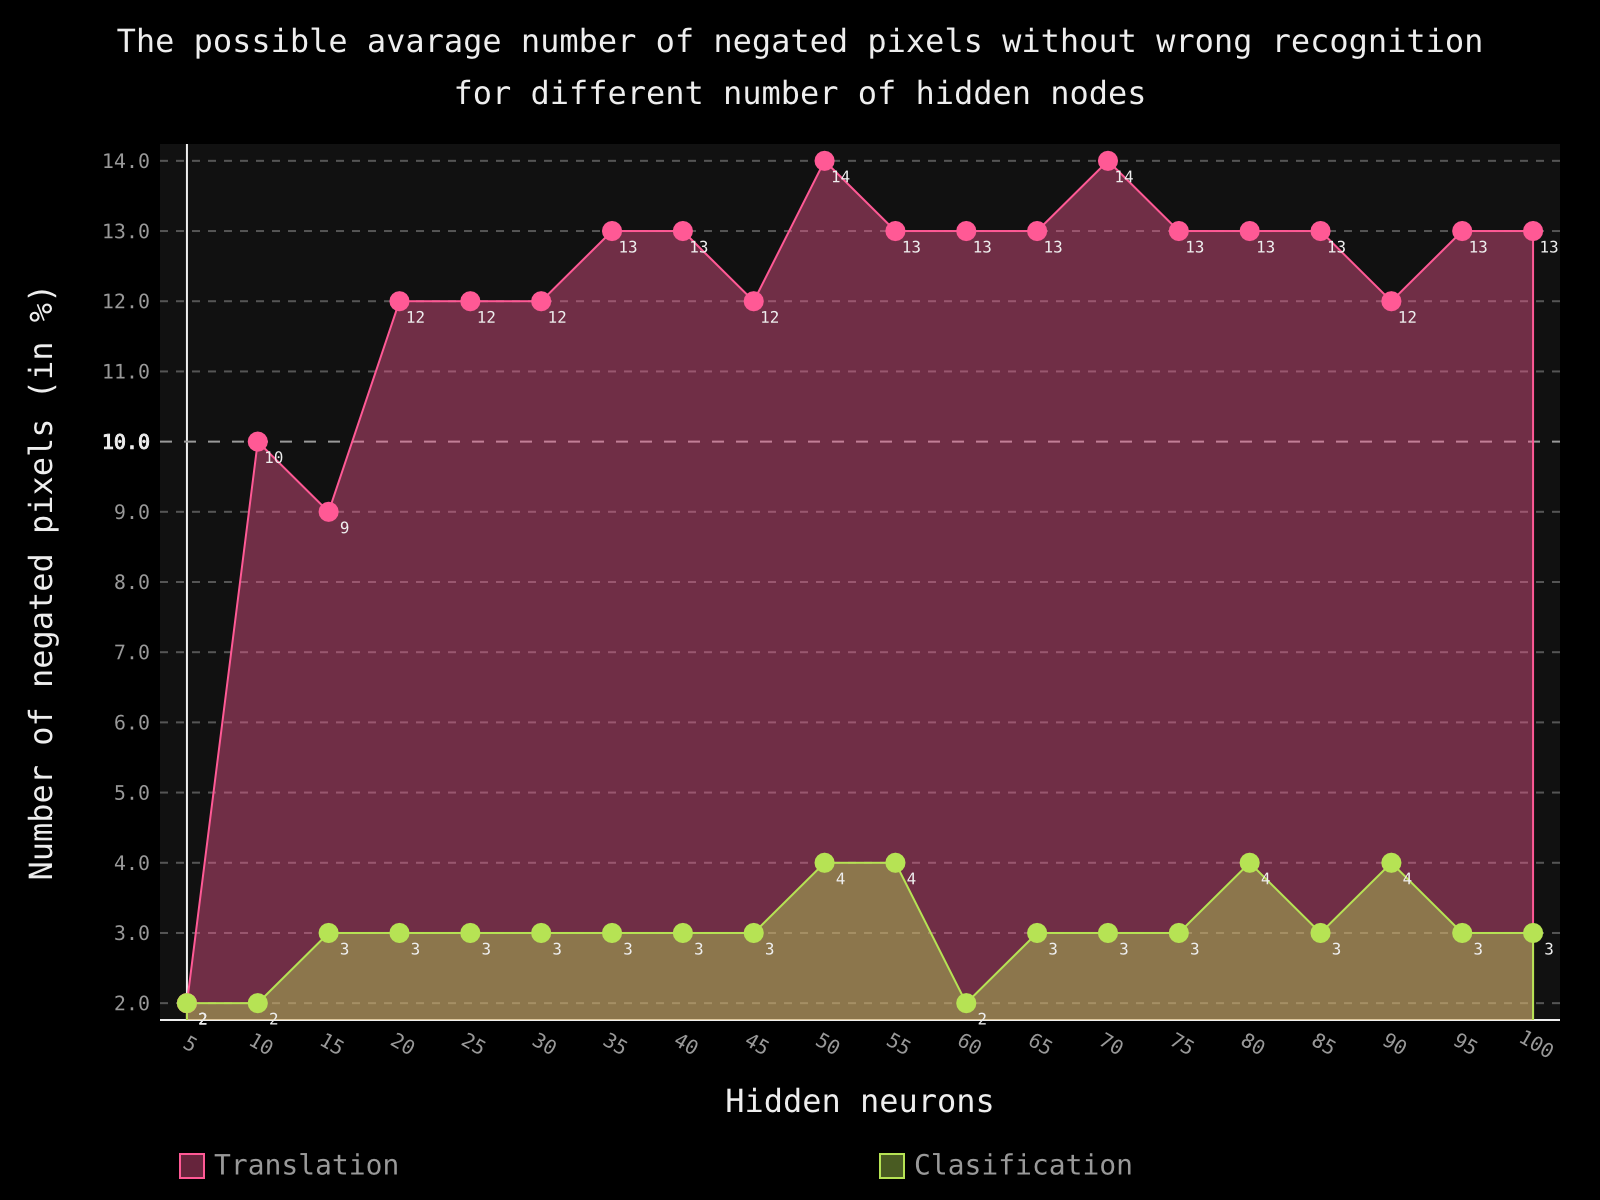
\includegraphics[scale=0.7,keepaspectratio=true]{Charts/hiddenChart.png}	
	\caption{}
	\label{hidden}
\end{figure} 

On figure \ref{learn} we can see that learning rate has no significant influence on later results, learning rate with value 0.016 was used for later tests.
\begin{figure}[h!]
	\centering
	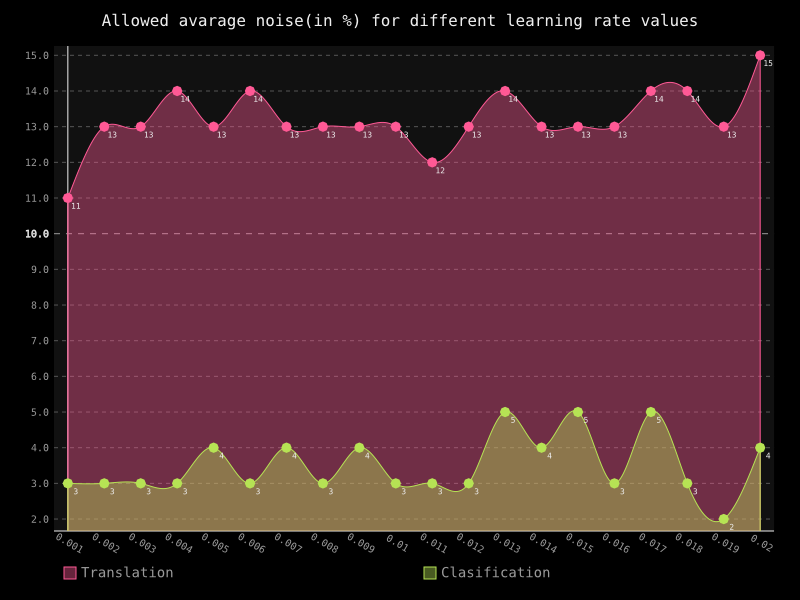
\includegraphics[scale=0.7,keepaspectratio=true]{Charts/learnChart.png}	
	\caption{}
	\label{learn}
\end{figure} 

Analizing chart on figure \ref{momentum} it can be seen that best value of momentum is oscilating aroung 0.95 and that value was chosen for later tests.
\begin{figure}[h!]
	\centering
	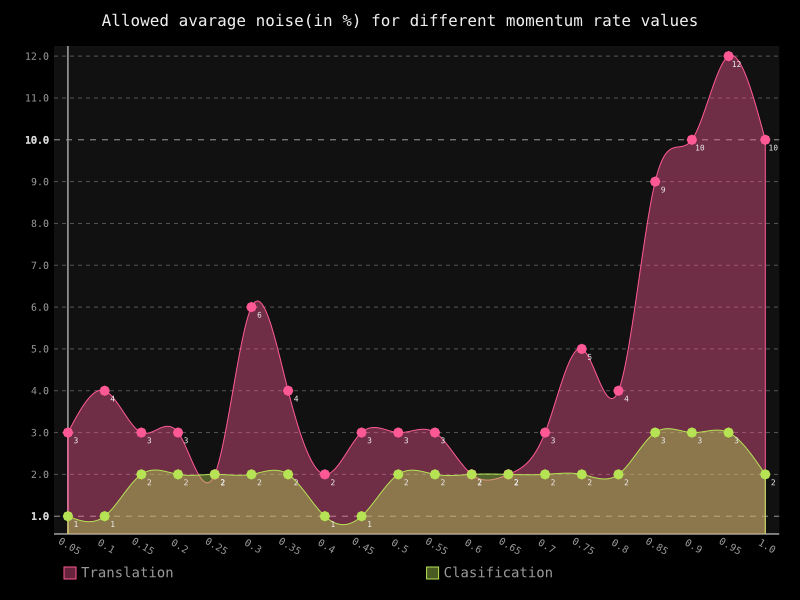
\includegraphics[scale=0.7,keepaspectratio=true]{Charts/momentumChart.png}	
	\caption{}
	\label{momentum}
\end{figure}

Final training was done with following parameters:
\begin{itemize}
	\item Training epochs: 55
	\item Number of hidden neurons: 55
	\item Learning rate: 0.016
	\item Momentum: 0.95
\end{itemize}

\section{Engine description}

After training and tests we decided to create Multilayer Perceptron with 1 hidden layer and 55 hidden neurons. During experiments it occured that the best results in case of clasification we get using softmax hidden and output layer type. For translation the best was sigmoid layer type so it was used.

\clearpage
\pagebreak
\section{Gained results}

\begin{figure}[h!]
	\centering
	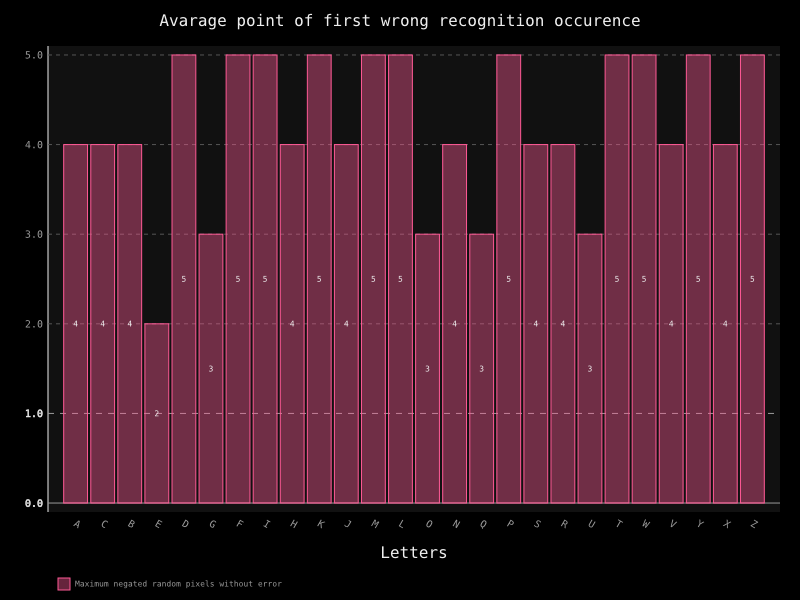
\includegraphics[scale=0.7,keepaspectratio=true]{Charts/RandNoiseTestPlanResultsChart_NormalTester.png}	
	\caption{}
	\label{noise_trans}
\end{figure}

\begin{figure}[h!]
	\centering
	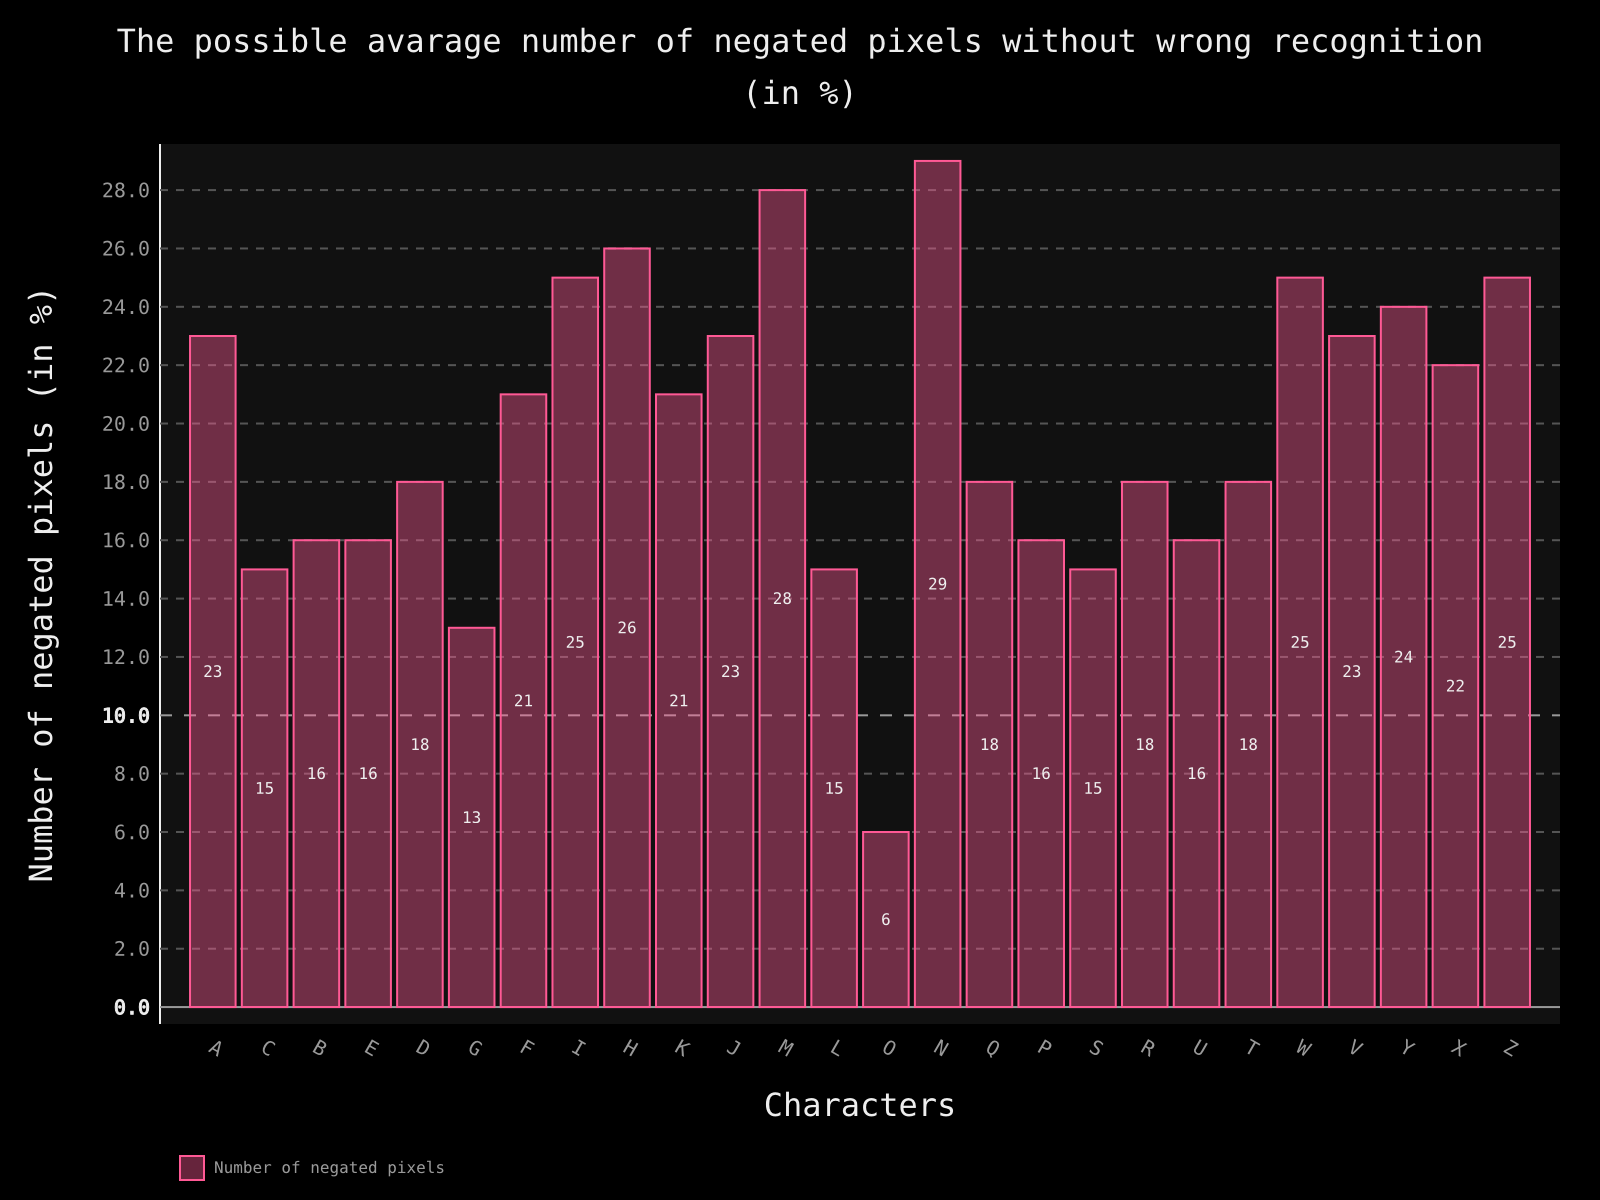
\includegraphics[scale=0.7,keepaspectratio=true]{Charts/RandNoiseTestPlanResultsChart_ClasifierTester.png}	
	\caption{}
	\label{noise_clas}
\end{figure}

\begin{figure}[h!]
	\centering
	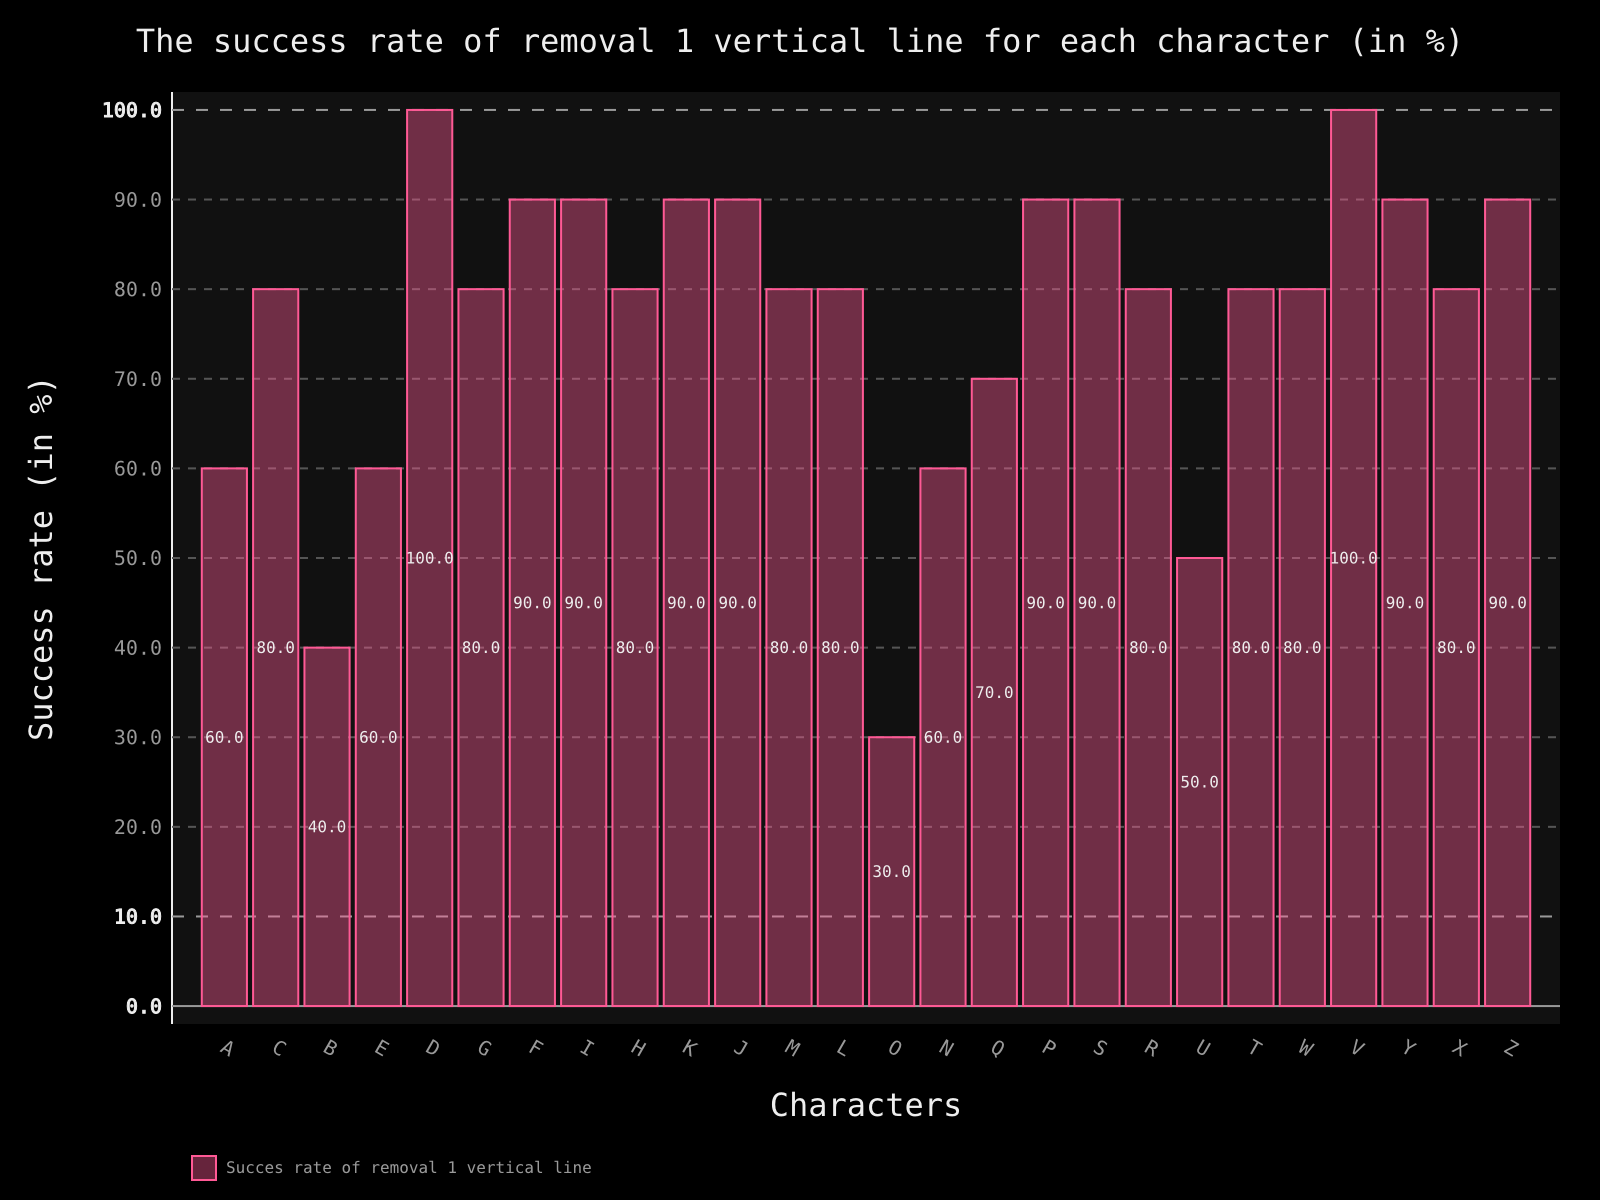
\includegraphics[scale=0.7,keepaspectratio=true]{Charts/VerLineTestPlanResultsChart_NormalTester.png}	
	\caption{}
	\label{ver_line_trans}
\end{figure}

\begin{figure}[h!]
	\centering
	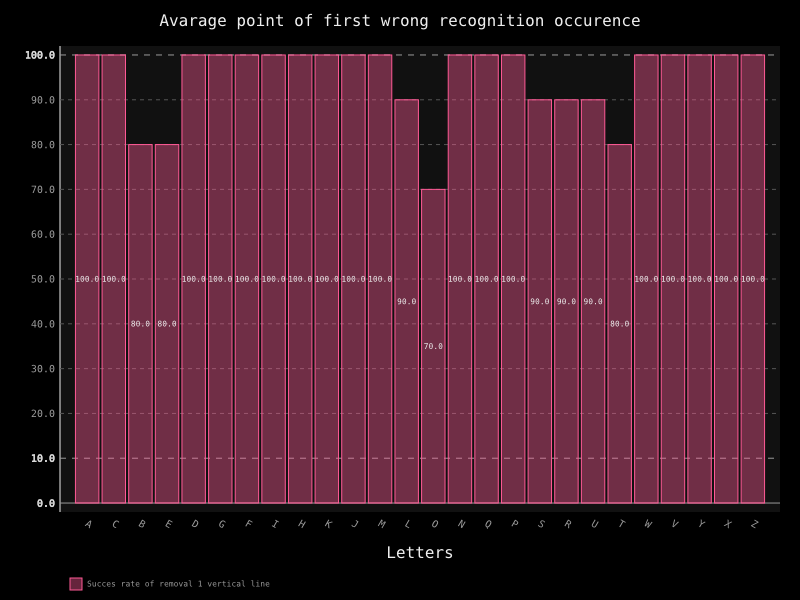
\includegraphics[scale=0.7,keepaspectratio=true]{Charts/VerLineTestPlanResultsChart_ClasifierTester.png}	
	\caption{}
	\label{ver_line_clas}
\end{figure}

\begin{figure}[h!]
	\centering
	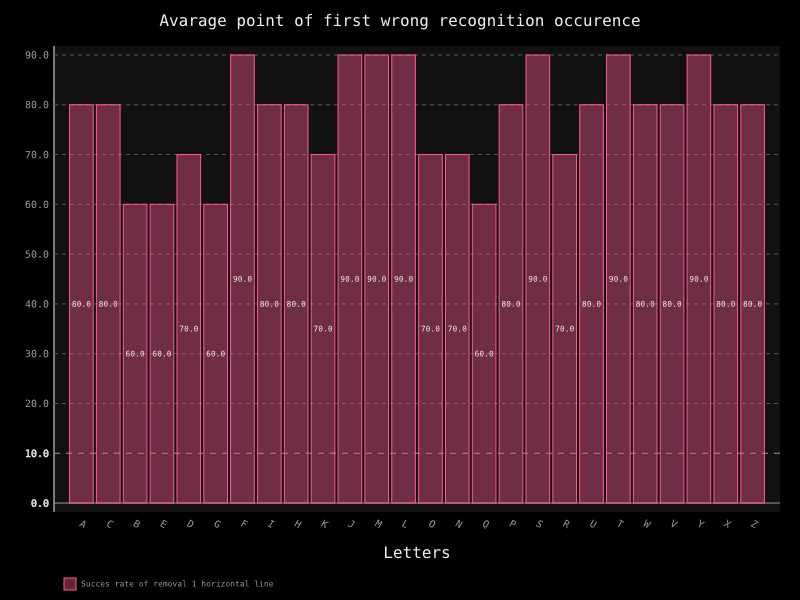
\includegraphics[scale=0.7,keepaspectratio=true]{Charts/HorLineTestPlanResultsChart_NormalTester.png}	
	\caption{}
	\label{hor_line_trans}
\end{figure}

\begin{figure}[h!]
	\centering
	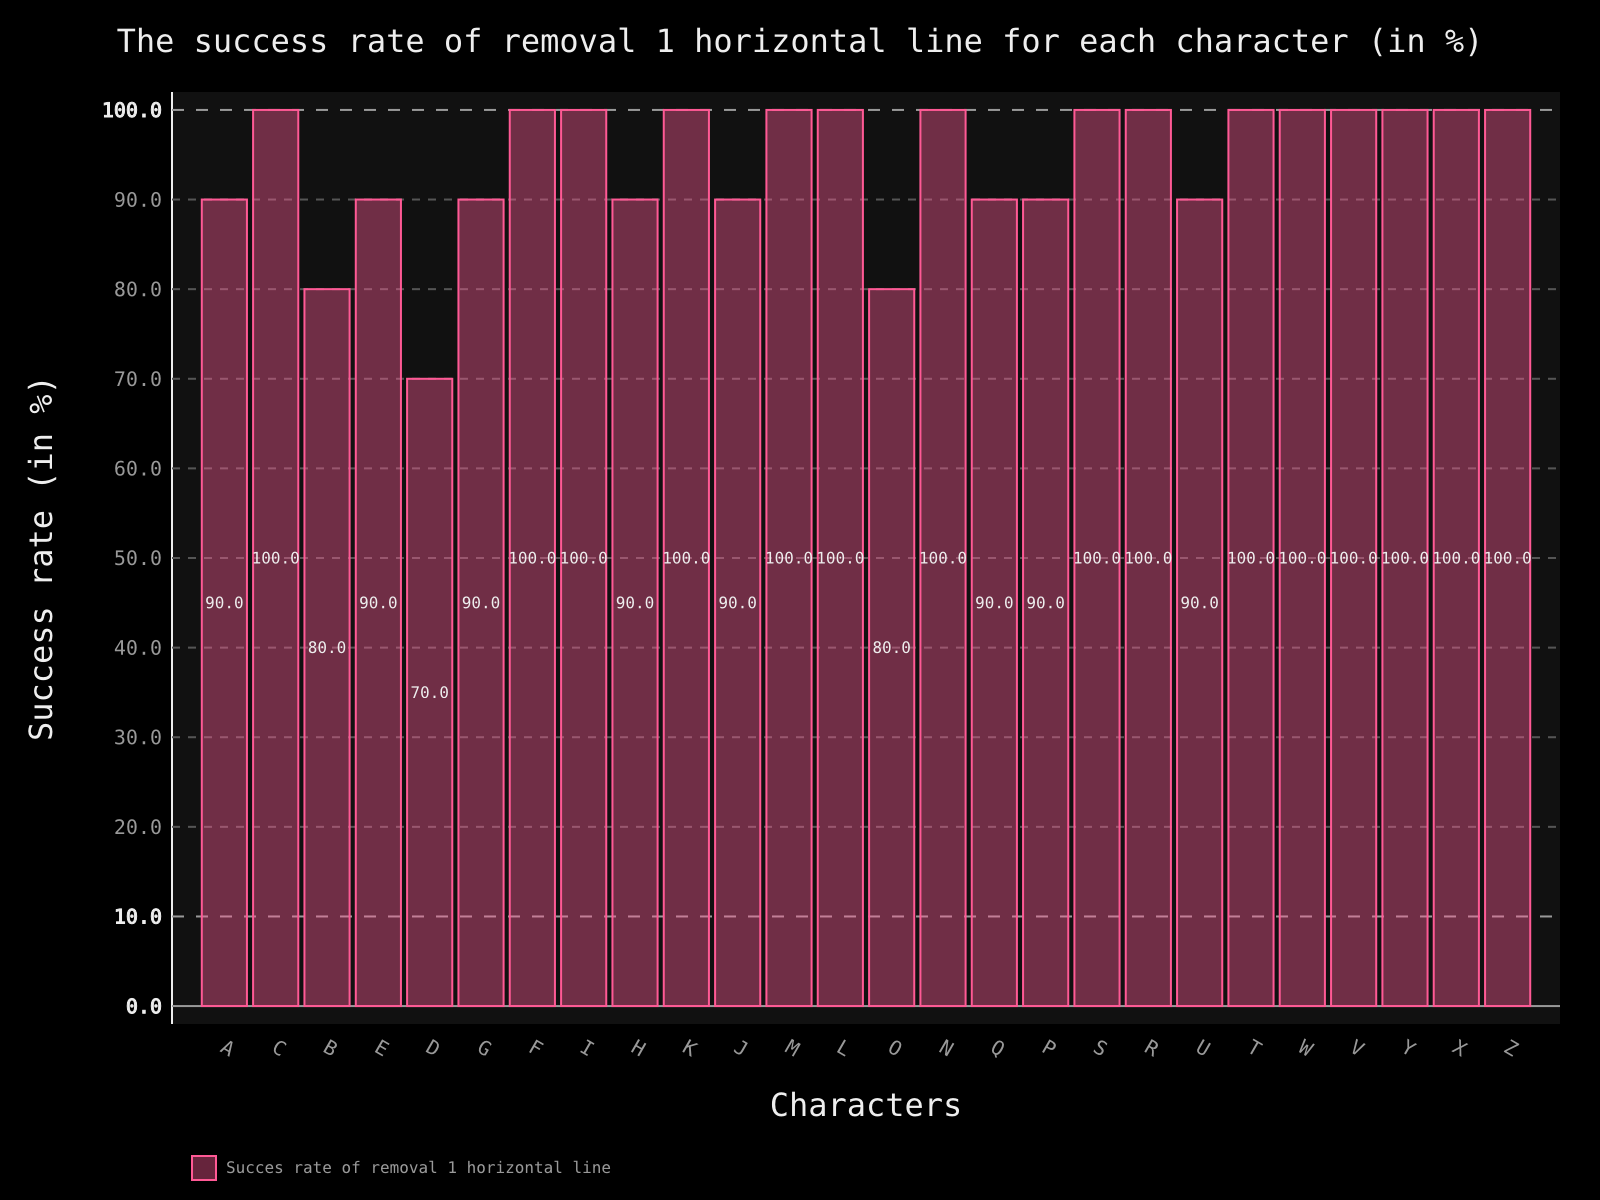
\includegraphics[scale=0.7,keepaspectratio=true]{Charts/HorLineTestPlanResultsChart_ClasifierTester.png}	
	\caption{}
	\label{hor_line_clas}
\end{figure}

\begin{figure}[h!]
	\centering
	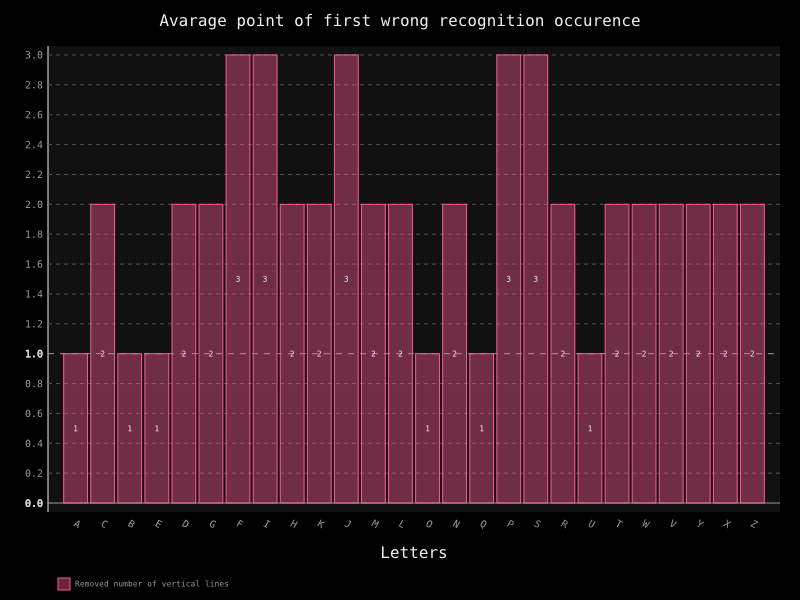
\includegraphics[scale=0.7,keepaspectratio=true]{Charts/LinesVerTestPlanResultsChart_NormalTester.png}	
	\caption{}
	\label{ver_lines_trans}
\end{figure}

\begin{figure}[h!]
	\centering
	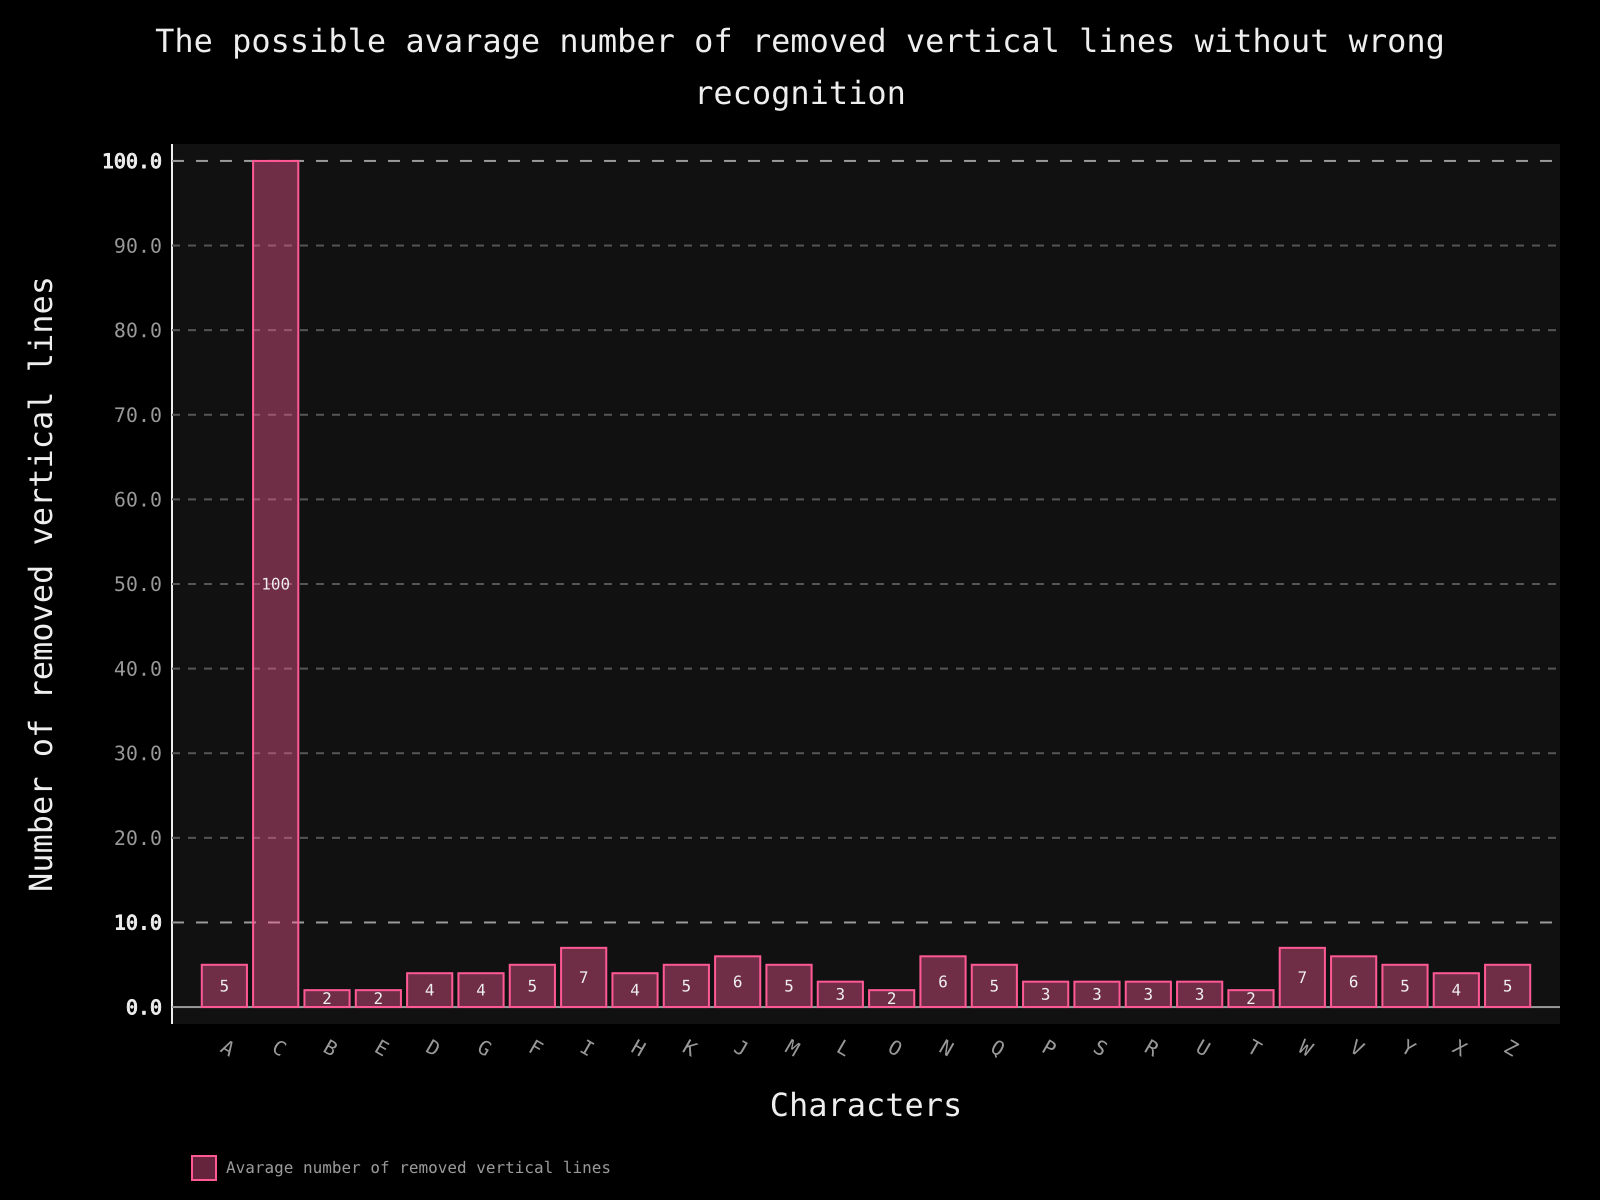
\includegraphics[scale=0.7,keepaspectratio=true]{Charts/LinesVerTestPlanResultsChart_ClasifierTester.png}	
	\caption{}
	\label{ver_lines_clas}
\end{figure}

\begin{figure}[h!]
	\centering
	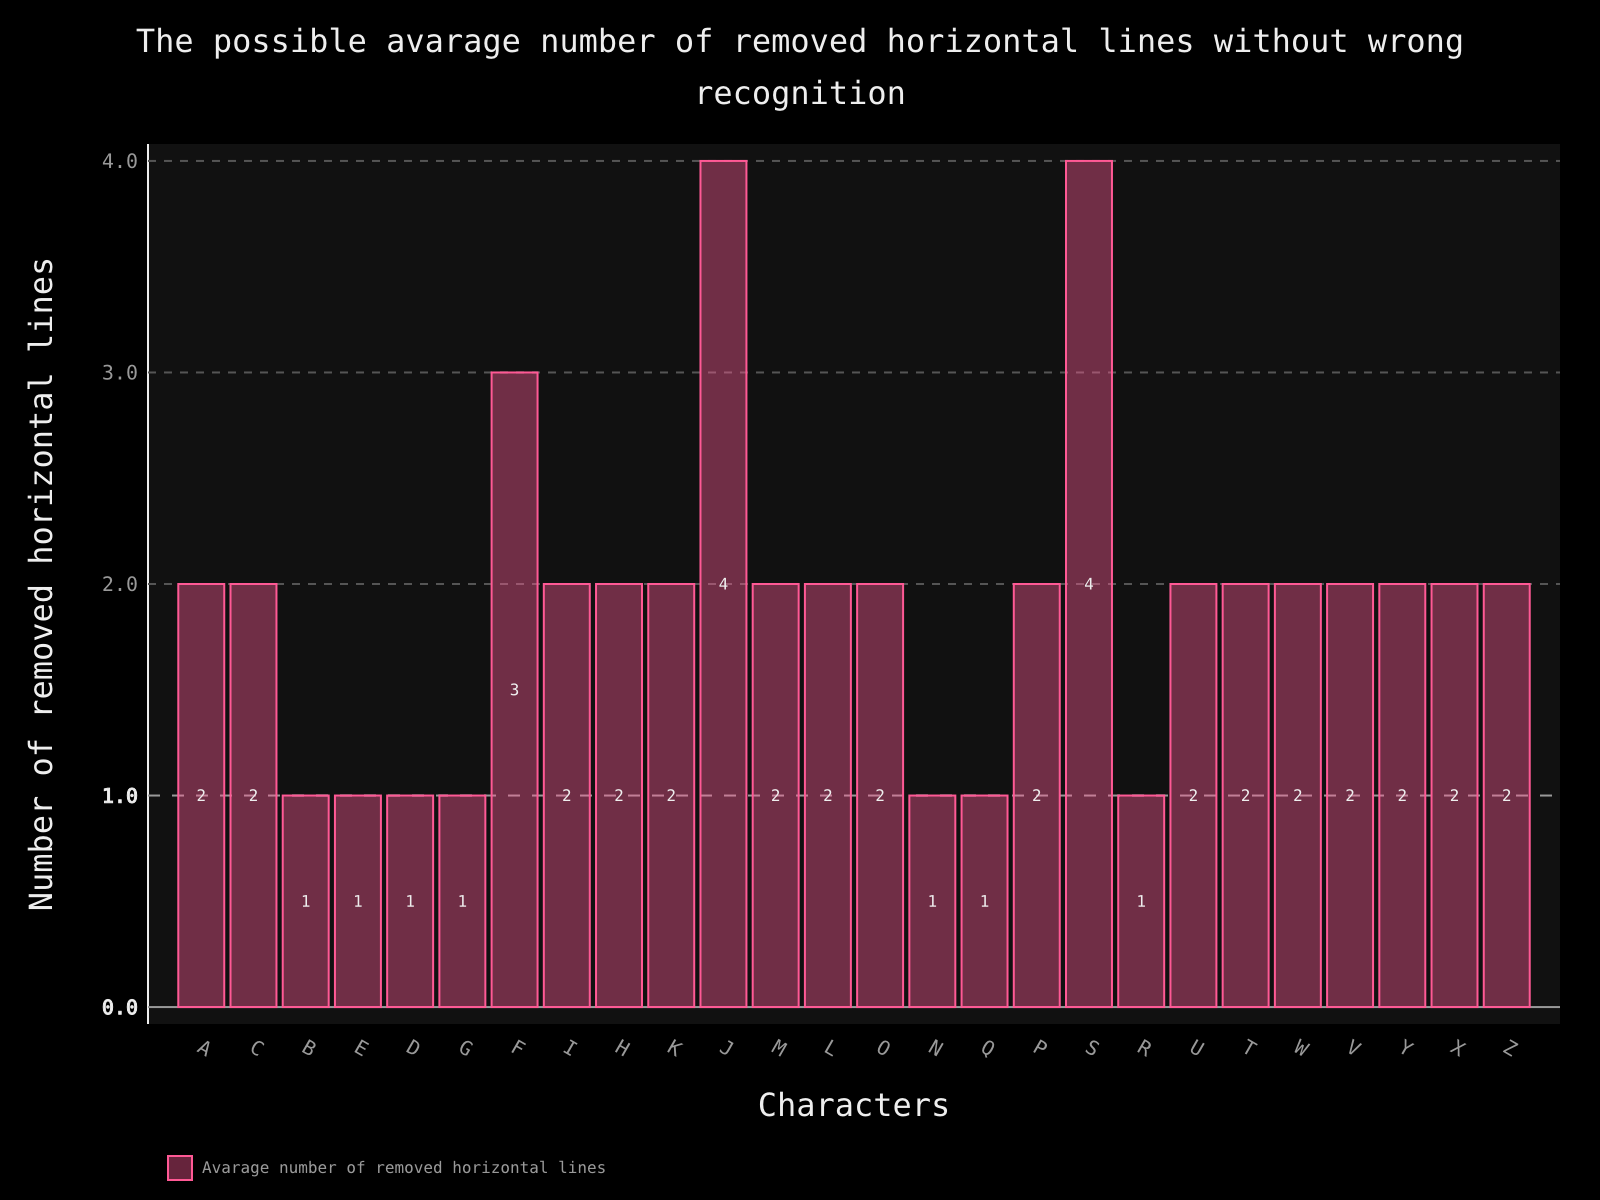
\includegraphics[scale=0.7,keepaspectratio=true]{Charts/LinesHorTestPlanResultsChart_NormalTester.png}	
	\caption{}
	\label{hor_lines_trans}
\end{figure}

\begin{figure}[h!]
	\centering
	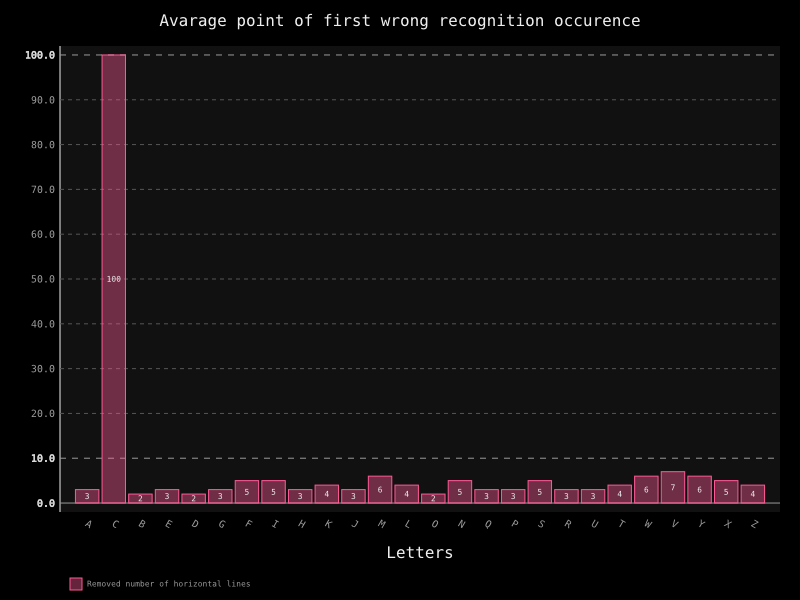
\includegraphics[scale=0.7,keepaspectratio=true]{Charts/LinesHorTestPlanResultsChart_ClasifierTester.png}	
	\caption{}
	\label{hor_lines_clas}
\end{figure}

\begin{figure}[h!]
	\centering
	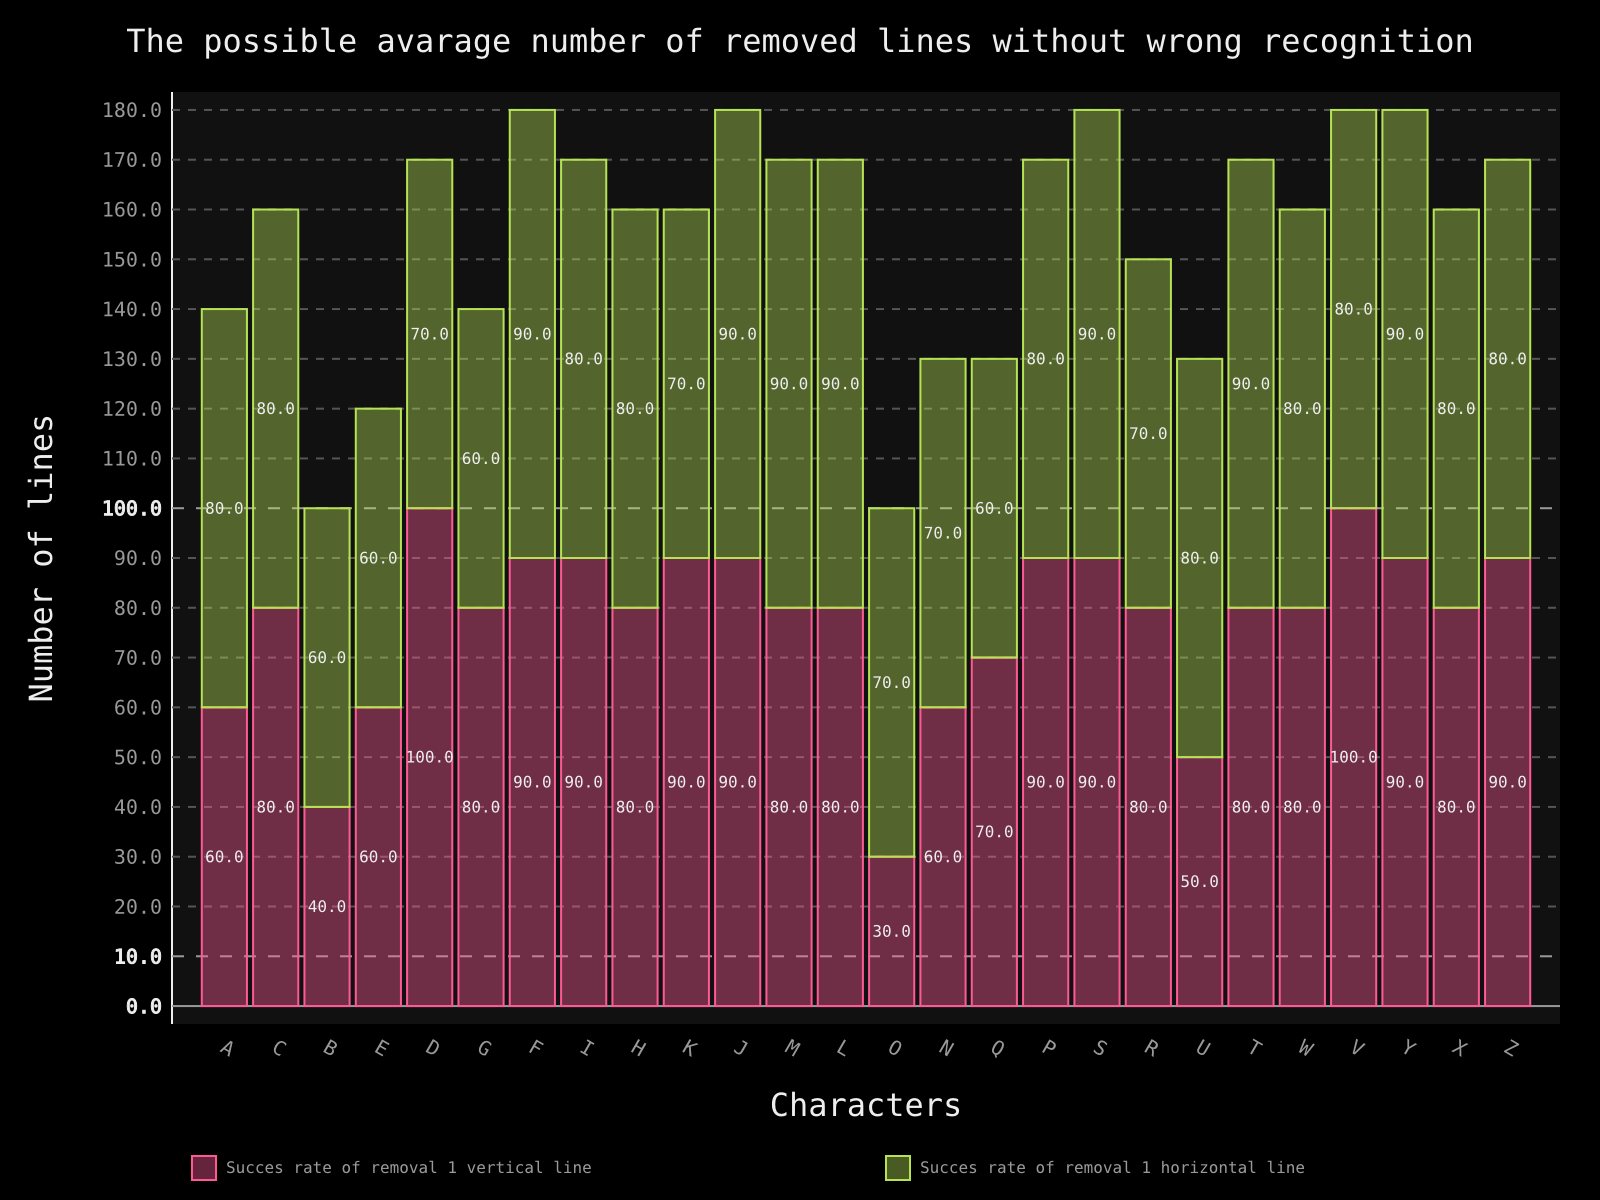
\includegraphics[scale=0.7,keepaspectratio=true]{Charts/Removed_linesTestPlanResultsChart_NormalTester.png}	
	\caption{}
	\label{lines_trans}
\end{figure}

\begin{figure}[h!]
	\centering
	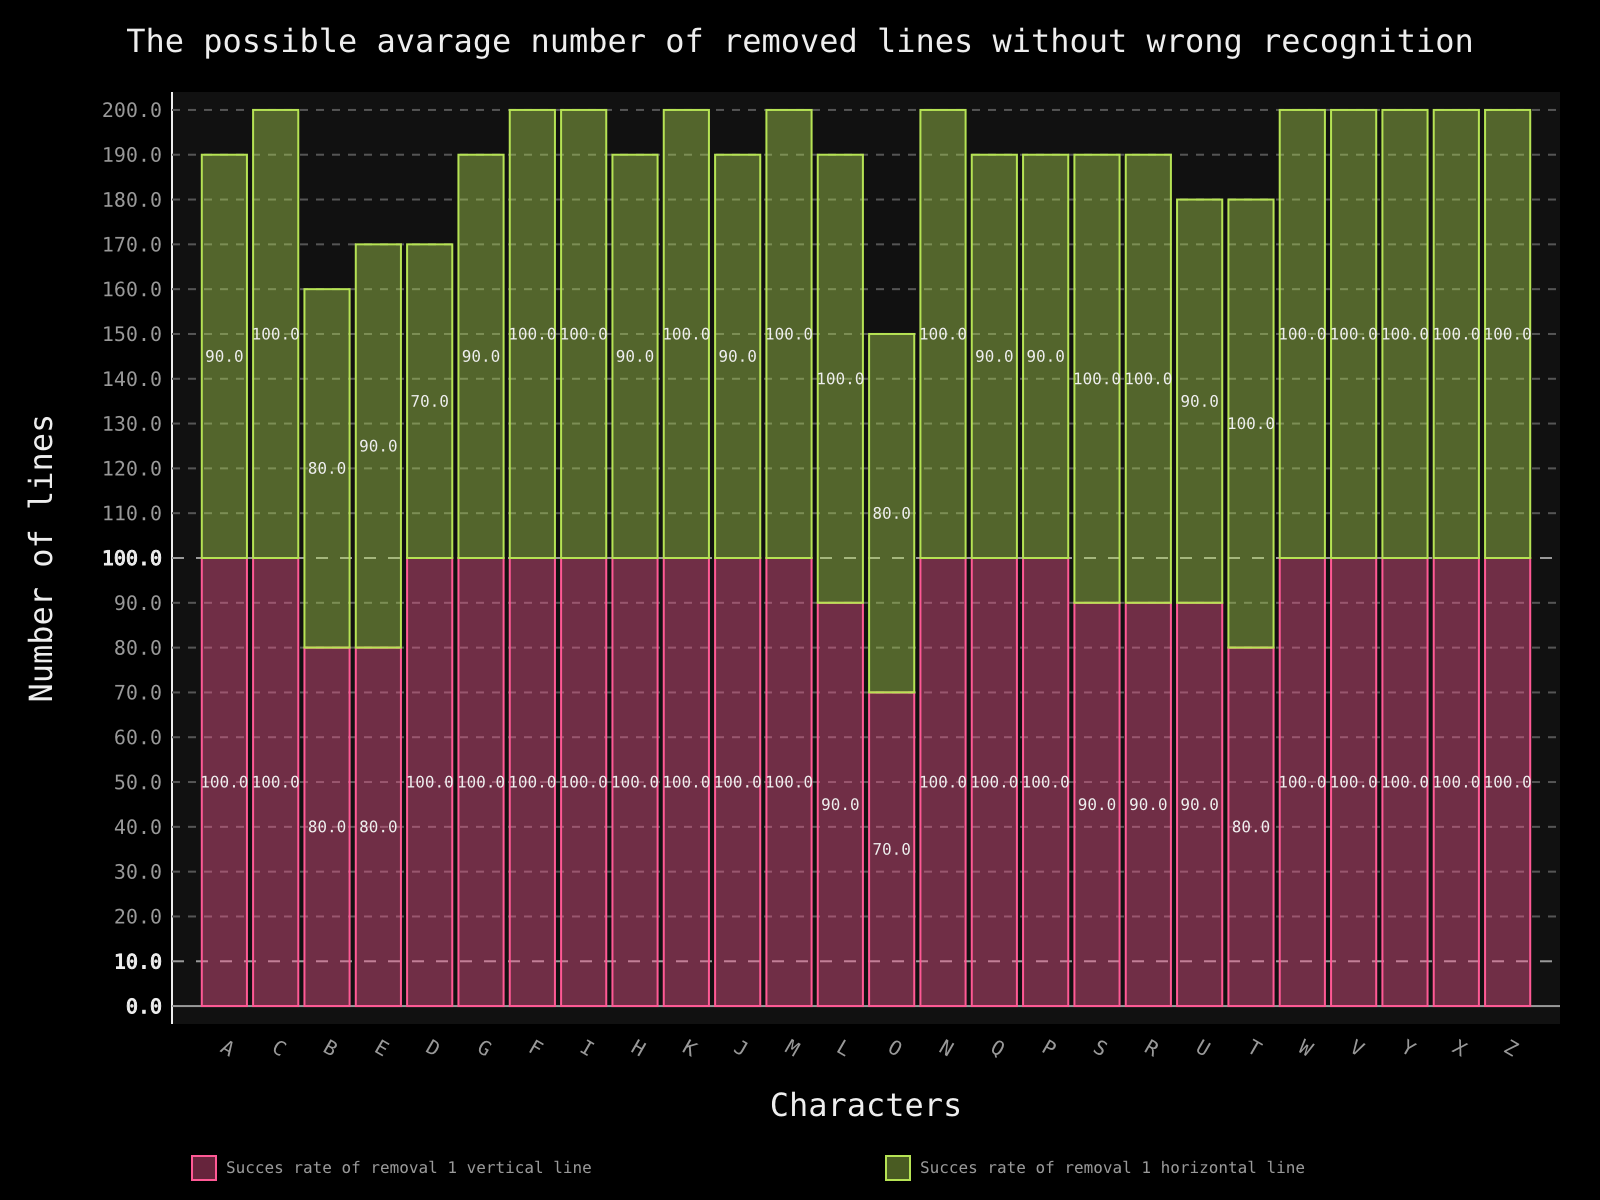
\includegraphics[scale=0.7,keepaspectratio=true]{Charts/Removed_linesTestPlanResultsChart_ClasifierTester.png}	
	\caption{}
	\label{lines_clas}
\end{figure}

\begin{figure}[h!]
	\centering
	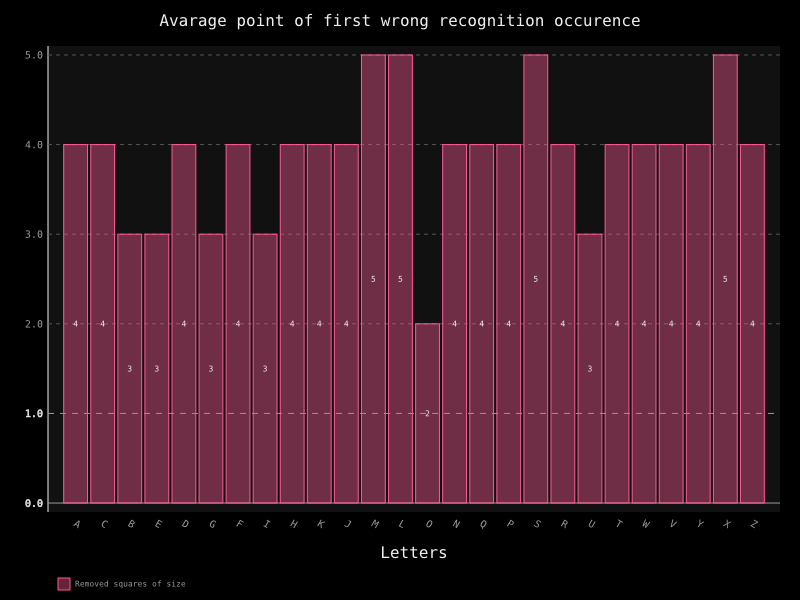
\includegraphics[scale=0.7,keepaspectratio=true]{Charts/SquaresTestPlanResultsChart_NormalTester.png}	
	\caption{}
	\label{squares_trans}
\end{figure}

\begin{figure}[h!]
	\centering
	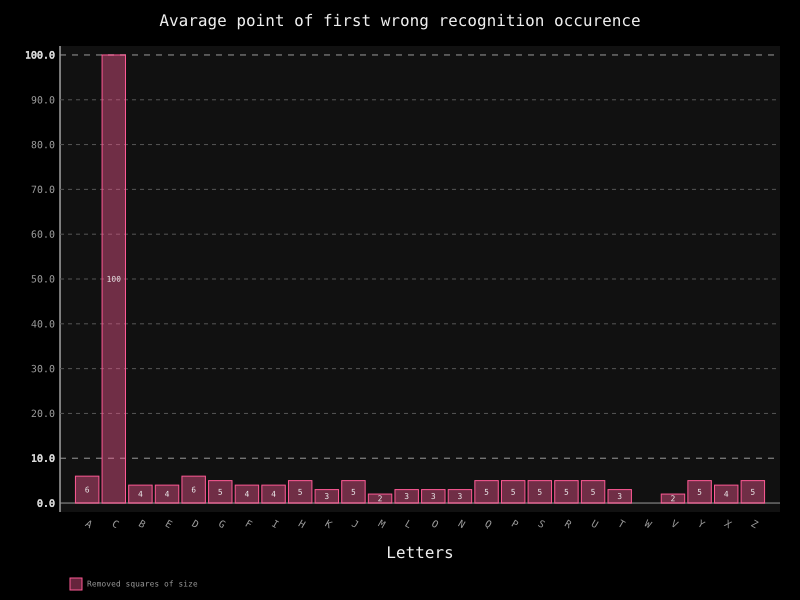
\includegraphics[scale=0.7,keepaspectratio=true]{Charts/SquaresTestPlanResultsChart_ClasifierTester.png}	
	\caption{}
	\label{squares_clas}
\end{figure}

\begin{figure}[h!]
	\centering
	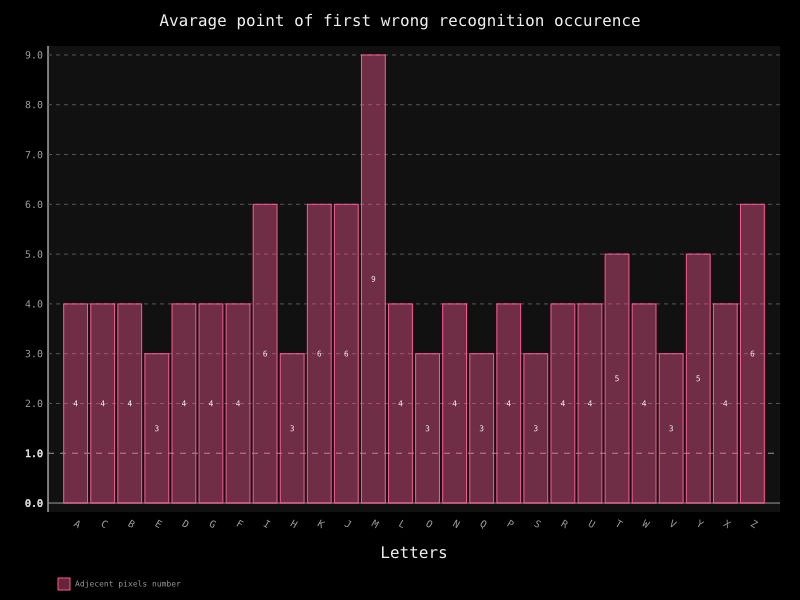
\includegraphics[scale=0.7,keepaspectratio=true]{Charts/AdjecentTestPlanResultsChart_NormalTester.png}	
	\caption{}
	\label{adjecent_trans}
\end{figure}

\begin{figure}[h!]
	\centering
	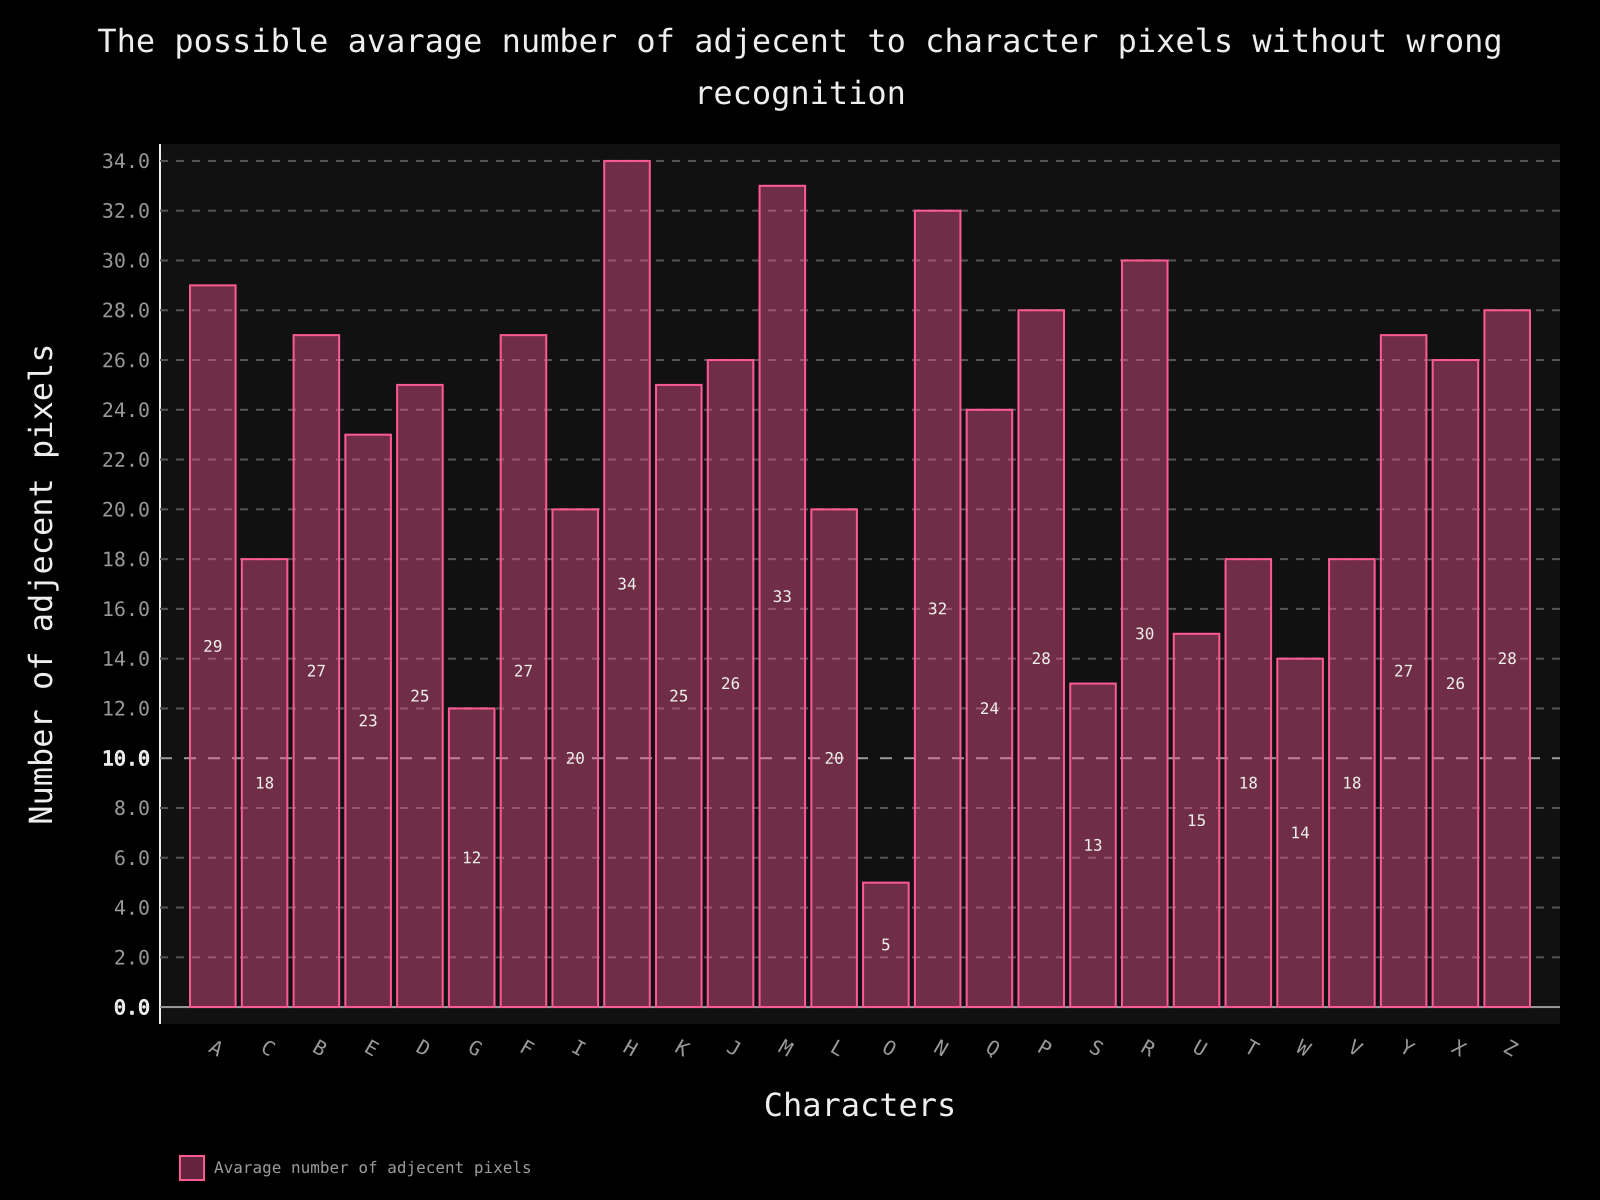
\includegraphics[scale=0.7,keepaspectratio=true]{Charts/AdjecentTestPlanResultsChart_ClasifierTester.png}	
	\caption{}
	\label{adjecent_clas}
\end{figure}

\begin{figure}[h!]
	\centering
	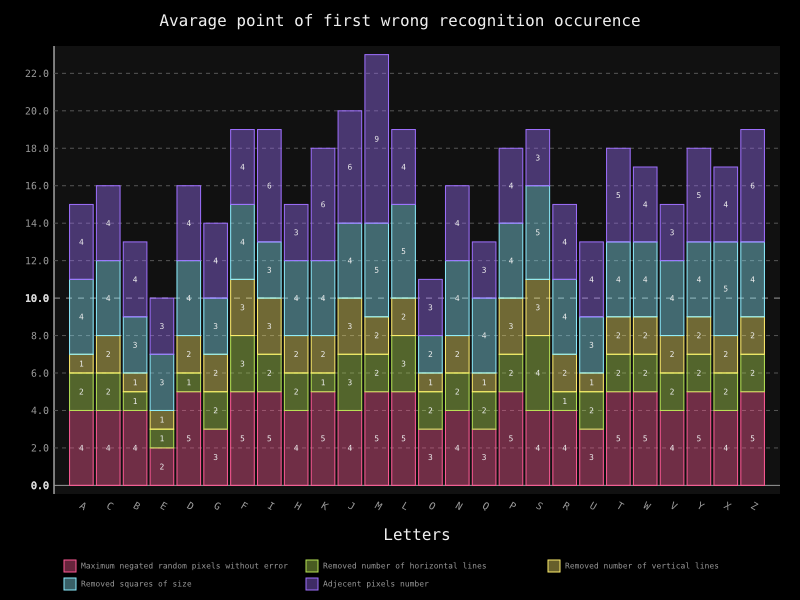
\includegraphics[scale=0.7,keepaspectratio=true]{Charts/AllTestPlanResultsChart_NormalTester.png}	
	\caption{}
	\label{all_trans}
\end{figure}

\begin{figure}[h!]
	\centering
	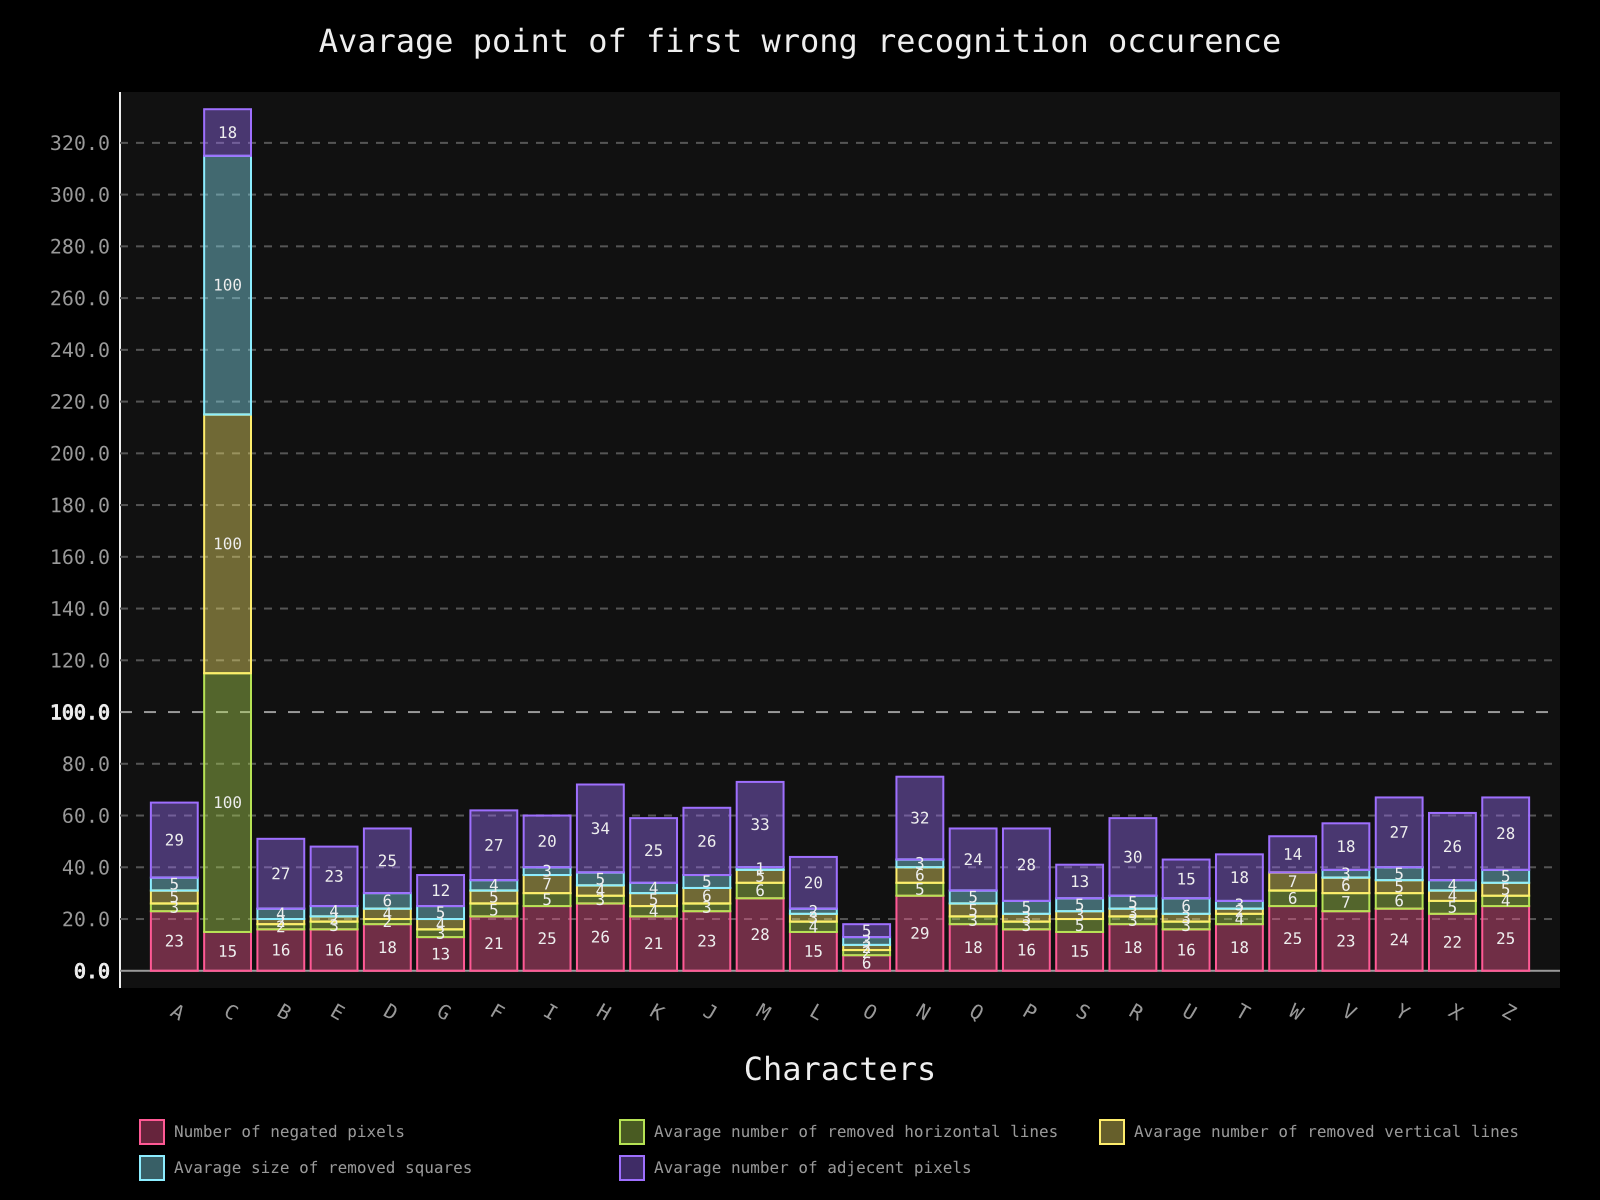
\includegraphics[scale=0.7,keepaspectratio=true]{Charts/AllTestPlanResultsChart_ClasifierTester.png}	
	\caption{}
	\label{all_clas}
\end{figure}
\pagebreak
\section{Final remarks}
It can be noticed that some characters are easier to be recognized by engine.
On figure \ref{all_trans} and \ref{all_clas} it is visible that letters like O, U, G are much sensible for different disortions. In the other hand letters like K, M, H, with many lines are resistant to them.
Because it is much easier for network to give proper output for one class per one output neuron it is visible that automatic clasification is much better than translation. There is no reson to use automatic translation because it gives much worse results tryng to recognize characters with different noises and distortions.
Summarizing we have to admit that results exceeded our expectations. Correct recognition of letter with almost 30\% of additional pixels which make character more bold or 30\% of random noise is a really big number and could make hard to recognize character even for human.

\end{document}
